% CREATED BY DAVID FRISK, 2016
\chapter{Theory}
\label{ch:theory}
This chapter will present the theory behind the construction of  a client and server verifiable additive homomorphic secret sharing construction presented in chapter \ref{ch:Methods}. First  the preliminaries are described, including notation, theorems, definitions, assumptions  and cryptographic preliminaries and concepts. Then the VAHSS construction \cite{SumItUp} \cite{VAHSS}, which this reports aims to extend to verify clients input is explained.  Finally two range proof and a set membership constructions is presented. 


\section{Preliminaries}
%TODO INTRO

\subsection*{Notation and setup}
To make the text more comprehensible notation that is used throughout the paper is introduced and defined here.  

%Consider $n$ clients and $m$ servers, to simplify notation define the two sets $\mathcal{N}=\{1,...,n\}$ and $\mathcal{M} = \{1,...,m\}$. Let $c_i$ and $x_i$ for $i\in\mathcal{N}$ denote the clients (data providers) and their respective data. Denote the servers by $s_j$, where $\:j\in\mathcal{M}$.


Let $\mathds{F}=\mathds{Z}_p$ denote a finite field, where $p$ is a large prime and let $\mathds{G}$ denote a unique subgroup of order $q$.  Define $g\in\mathds{G}$ to be a group generator and $h\in\mathds{G}$ a group element such that  $log_g\:h$ is unknown and $h$ co-prime to $p$. 

The notation $y\in_R\mathds{Y}$, means that an element $y$ in chosen at random from the set $\mathds{Y}$.

\subsection*{Definitions, Theorems and Assumptions}
The discrete logarithm assumption and q-strong Diffie Hellman assumption define below does not hold in the presence of quantum computers. All cryptographic constructions presented in this paper relies on one or both of these two assumptions, hence the security is not guaranteed post quantum. 
\vspace{10pt}
\begin{Mydef}[\textbf{Pseudorandom Function (PRF)}]
Let $S$ be a  distribution over $\{0,1\}^l$ and $F_s\: :\: \{0,1\}^m\to\{0,1\}^n$ a family of functions indexed by a string $s$ in the support $S$. It is defined that $\{F_s\}$ is a pseudo random function family if, for every PPT adversary $\mathcal{A}$, there exists a negligable function $\varepsilon$ such that:
\begin{align*}
|\text{Pr}[\mathcal{A}^{F_s}(\cdot) = 1] - \text{Pr}[\mathcal{A}^{R}(\cdot) = 1] | \leq \varepsilon,
\end{align*}
where $s$ in distributed according to $S$ and $R$ is a function sampled uniformly at random from the set of all functions mapping from $\{0,1\}^n$ to $\{0,1\}^m$.
\end{Mydef}
\vspace{10pt}
\begin{Mydef}[\textbf{Euler's totient function}]
The function $\Phi(n)$ is defined as the counter of the number of integers that are relative primes to $n$ in the set $\{1,...,n\}$ . Note if $n$ is a prime number $\phi(n) = n-1$.
\end{Mydef}
\vspace{10pt}
\begin{thm}[\textbf{Euler's Theorem}]
\label{thm:euler}
For all integers $x$ and $n$ that are co-prime it holds that:
$x^{\Phi(n)} = 1\:( \text{mod n})$, where $\Phi(n)$ is Euler's totient function.
\end{thm}
\vspace{10pt}
From Theorem \ref{thm:euler} it follows that for arbitrary $y$ it holds that $x^{y\Phi(n)} = 1 \:( \text{mod n})$.
\vspace{10pt}

\begin{Ass}[\textbf{Discrete logarithmic assumption}]
\label{ass:DLA}
Let $\mathds{G}$ be a group of prime order $q$, a generator $g\in \mathds{G}$ and an arbitrary element $y \in\mathds{G}$, it is  infeasible to find $x \in \mathds{Z}_q$, such that $y=g^x$
\end{Ass}

\vspace{10pt}
\begin{Ass}[\textbf{q-strong Diffie Hellman Assumption}]
 Given a group $\mathds{G}$, a random generator $g\in \mathds{G}$ and powers $g^x,...,g^{x_q}$, for $x \in_R \mathds{F}$ and  $q= |\mathds{G}|$. It is then  infeasible for an adversary to find $(c, g^{\frac{1}{x+c}})$, where $c \in \mathds{F}$.
\end{Ass}




\subsection*{Homomorphic Secret Sharing}
Secret sharing, first mentioned in \cite{How_share_A_secret}, hides a secret $x$ by splitting it into shares, where any subset $\mathcal{S}$ of shares smaller than a threshold $\tau$, i.e $|\mathcal{S}|<\tau$, reviles no information about the original value of $x$.  Let a secret $x$ be split into $m$ shares denoted $x_i \text{ s.t } i\in\{1,...,m\}$, then in order to reconstruct the value $x$ at least $\tau$ shares has to be combined, this is called a $(\tau,m)$-threshold scheme. I  this paper the threshold will be equal to the number of shares,  $\tau=m$. and additive secret sharing scheme  will be considered. Additive secret sharing means that to reconstruct the secret at least $\tau$ shares are added, $x = \sum_{i=1}^\tau x_i$.

\subsection*{Homomorphic hash functions}
Let $\mathcal{H}$ be a cryptographic hash function, $\mathcal{H}:\mathds{F}\mapsto \mathds{G}$. Any such function should satisfy the following two properties:
\begin{itemize}
    \item \textbf{Collision-resistant} It should be hard to find $x,x'\in\mathds{F}$ such that $x\neq x'$ and $\mathcal{H}(x)=\mathcal{H}(x')$.
    \item \textbf{One-Way} It should be computationally hard to find $\mathcal{H}^{-1}(x)$.
\end{itemize}

A homomorphic hash function should also satisfy the following property:
\begin{itemize}
    \item \textbf{Homomorphism} For any $x,x'\in\mathds{F}$ it should hold that $\mathcal{H}(x\circ x') = \mathcal{H}(x)\circ\mathcal{H}(x')$. Where $\circ$ is either $"+"$ or $"*"$.
\end{itemize}

A such function satisfying the thee properties is $\mathcal{H}_1(x):\mathds{F}\mapsto\mathds{G}$ and $\mathcal{H}_1(x)= g^{x}$ \cite{HHF}. 


\subsection*{Pedersen Commitment scheme}
A commitment to a secret $x\in\mathds{F}$ is the \textit{Pedersen commitment scheme} defined as $\mathds{E}(x,R)=g^xh^R$, where $R\in_R\mathds{F}$,  originally presented in \cite{pedersen}. This commitment satisfies the following theorem;
\\
\begin{thm}
\label{thm:C=g^xh^R}
For any $x\in\mathds{F}$ and for $R\in_R\mathds{F}$, it follows that   $\mathds{E}(x,R)$ is uniformly distributed in $\mathds{G}$. If we have two commits satisfying $\mathds{E}(x,R)=\mathds{E}(x',R')$  $x\neq x'$ and  $x\neq x'$ then it must hold that $R\neq R' \:\text{mod}\:q$ and 
\begin{equation}
\label{eq:pedersen_binidng}
    log_g(h) = \frac{x-x'}{R'-R} \text{ mod }N.
\end{equation}
\end{thm}
\begin{proof}
The statements of the theorem follows from solving for $log_g(h)$ in $\mathds{E}(x,R)=\mathds{E}(x',R')$ 
\end{proof}

Theorem \ref{thm:C=g^xh^R} implies that if someone knows the discrete logarithm of $h$ with respect to $g$, i.e $log_g(h)$, this person is able to provide two equal commits, $\mathds{E}(x,R)=\mathds{E}(x',R')$ such that $x\neq x'$. However the $log_g h$ is assumed to be unknown hence it is not possible to construct two equal commits hiding different secrets. This means that the Pedersen commitment scheme is computational binding under the discrete logarithm assumption, it is also perfectly hiding of the secret $x$ \cite{pedersen}. 

Further note that Pedersen commitment is homomorphic. Hence for arbitrary messages $x_1,x_2\in\mathds{F}$, random values $R_1,R_2\in_R\mathds{F}$ and the commits $C_i=\mathds{E}(x_i,R_i),\:i\in\{1,2\}$, it holds that $C_1\cdot C_2 = \mathds{E}(x_1+x_2,R_1+R_2)$.

A final remark about the Pedersen commitment is the similarity between the hash function $\mathcal{H}_1$ and the Pedersen commitment $\mathds{E}$, the hash function can be seen as a generalisation of the Pedersen commitment. This will be used later when including verification of client to the VAHSS construction.

A Pedersen commitment scheme can also be defined for vectors and is then called \textit{Pedersen vector commitment}. Lets consider a $n$ dimensional vector $\mathbf{x}\in\mathbf{F}^n$, let $\mathbf{g}=(g_1,...,g_n) \in\mathds{G}^n$ and $h\in\mathds{G}$ where $\mathds{G}$ is a group of order $p$ as above. A commitment to the vector  $\mathbf{x}=(x_1,...,x_n)$  with the random value $R\in_R \mathds{F}$ is then defined as $\mathds{E}(\mathbf{x},R) = \mathbf{g}^\mathbf{x}h^R = h^R\prod_{i=1}^n g_i^{x_i}$ and the commitment is a value in the one-dimensional group $\mathds{G}$. 

\subsection*{Bilinear mapping}
\label{sec:bilinear}
Bilinear mapping (also commonly refereed to as bilinear pairing) maps two group elements from one group to an element in another group. In this paper admissible bilinear mapping fulfilling Definition \ref{def:AdmissibleBM} will be used. In the definition given here two elements from the same group are mapped to another group, generally the definition of admissible bilinear maps two elements from different groups to a third group, i.e $e: \: \mathds{G}_1\times \mathds{G}_1 \to \mathds{G}_T$, but in this paper it will always hold that $\mathds{G}_1=\mathds{G_2}$ and hence the definition is given on this form. 
\begin{Mydef}[\textbf{Admissible Bilinear Map}]
	\label{def:AdmissibleBM}
	Let $\mathds{G}_1,\mathds{G}_T$ be two multiplicative cyclic groups of prime order $p$ such that there exist an admissible bilinear map $e: \: \mathds{G}_1\times \mathds{G}_1 \to \mathds{G}_T$. Let $\mathds{G}_1^*=\mathds{G}_1\backslash \{1\}$.  Then the bilinear map $e$ fulfils:
	\begin{itemize}
		\item Bilinear: for any group element  $g\in\mathds{G}_1^*$ and $a,b \in \mathds{Z}_p$,
		\begin{align*}
			e(g^a,g^b) = e(g,g)^{ab}
		\end{align*}	
		\item Non-degenerated: $e(g,g)\neq 1$	 
		\item The bilinear map is efficiently computable
	\end{itemize}
\end{Mydef}

The bilinear property of the mapping $e$ will later be used to create digital signatures and the idea to  behind is explained briefly.  Bohen-Boyen presented a a signature scheme that exploits the bilinear property of the mapping $e$ to verify the signatures \cite{Bohen-Boyen}. Shorty the scheme is constructed as, the signer knows the secret key $x$ and distributed the public key $g^x$, then to sign a message $m$ computes $\sigma = g^{1/(x+m)}$, this signature is $q-secure$ to forgery under the q-Strong Diffie Hellman Assumption. Verification is done by checking that $e(\sigma,y\cdot g^m) = e(g,g)$, which holds due to the bilinearity of $e$. 


\subsection*{Zero knowledge proof}
Zero-knowledge proofs (ZKP) is a cryptographic primitive that was first presented in \cite{OG_ZKP}. The idea behind a ZKP is that after successfully performing a ZKP a certain statement about a secret $x$ has been verified to be true (or false) without having revealed any other information about the secret $x$ beyond the statement. Here non interactive ZKP that ensures proof of knowledge (PoK) is of interest. Before closer defining what this means lets consider the set up and environment of ZKP protocol. A ZKP consists of two parties a \textit{prover} and a \textit{verifier}, further assume both parties has access to the protocol parameters generated by a set up algorithm and a language $\mathcal{L}\in \text{ NP}$, additionally the prover know a secret $x\in \mathcal{L}$. The prover constructs a proof that $x$ belongs to $\mathcal{L}$, by using a witness $w$ of $x$, then the verifier can in polynomial time determine if the proof is valid or not. 
For a ZKP to be non-interactive means that there is no communication required between the prover and verifier during the construction of the proof and PoK means that the verifier is not only convinces there exist a witness $w$ but also that the prover knows such a witness. A ZKP should fulfil the thee properties defined in Definition \ref{def:ZKP}, these definitions informally means that, a correctly constructed proof of an instance $x\in\mathcal{L}$ should be accepted with probability $1$, an incorrect constructed proof of an instance $x\notin\mathcal{L}$ should have a negligible probability of being accepted and the verifier should learn nothing about the secret beyond the statement being proved.
 

\begin{Mydef}
\label{def:ZKP}
First define the two algorithms;  \texttt{Prove}$(x,w)$ to be the algorithm for generating a ZKP of instance $x\in\mathcal{L}$ and witness $w$, and  \texttt{Verify} to be the verification algorithm of the correctness of the ZKP. Such a ZKP scheme  should fulfil the three properties: 
\begin{itemize}
\item \textbf{Completeness} Given a witness $w$ satisfying the instance $x\in\mathcal{L}$, it should hold that \texttt{Verify}$($\texttt{Prove}$(x,w)) = 1$. 
\item \textbf{Soundness} If the witness $w$ does not satisfy the  instance $x\notin\mathcal{L}$, then the probability  Prob$[$\texttt{Verify}$($\texttt{Prove}$(x,w)) = 1] < \varepsilon$, for a sufficiently small $\varepsilon$. 
\item  \textbf{Zero-knowledge} A proof system is \textit{honest verifier zero-knowledge} if there exist a PPT algorithm \texttt{Simulator} having access to the same input as the algorithm \texttt{Verify} but not the provers input, such that output from the \textt{Simulator} and \texttt{Prove} is indistinguishable, i.e have the same distribution given that $x\in\mathcal{L}$.  
\end{itemize}
\end{Mydef}
 
This paper will consider zero knowledge range proof (ZKRP) and zero knowledge set membership proofs (ZKSM) where the statement that the prover convinces the verifier of is that the secret belongs to a predetermined range or set.


\subsection*{Fiat-Shamir heuristic}
 Fiat-Shamir heuristic \cite{Fiat-Shamir} can be used to convert an interactive protocol into non interactive, here it will be used to construct non-interactive ZKP. A non interactive  ZKP requires no communication between the prover and verifier during the construction of the proof. In Interactive constructions the verifier sends a challenge $c\in_R\mathds{F}$ to the prover that is included in the proof in order to convince the verifier that the prover did not cheat. The Fiat-Shamir heuristic replaces the random challenge sent by the verifier with the output of a hash-function of the partial-proof up to this point. The Fiat-Shamir heuristic converts an interactive ZKP to non-interactive while preserving security and full zero-knowledge relying on the random oracle model (ROM). 

\section{Verifiable additive homomorphic secret sharing}
\label{sec:VAHSS}
%Consider $n$ clients and $m$ servers, to simplify notation define the two sets $\mathcal{N}=\{1,...,n\}$ and $\mathcal{M} = \{1,...,m\}$. Let $c_i$ and $x_i$ for $i\in\mathcal{N}$ denote the clients (data providers) and their respective data. Denote the servers by $s_j$, where $\:j\in\mathcal{M}$.

This section will describe a verifiable additive homomorphic secret sharing (VAHSS) Lets assume  $n$ clients/data providers and $m$ servers, to simplify notation define the two sets $\mathcal{N}=\{1,...,n\}$ and $\mathcal{M} = \{1,...,m\}$. Let $c_i$ and $x_i$ for $i\in\mathcal{N}$ denote the clients (data providers) and their respective data. Denote the servers by $s_j$, $\:j\in\mathcal{M}$. The idea of VAHSS is that each client split their secret $x_i$ into $m$ shares, denoted $x_{ij}$ and sends one share to each server. The servers receives shares from all $n$ clients and computes the partial sum $y_j = \sum_{i=1}^n x_{ij} $ and publishes the result. The final sum is then computed by summing the partial sums, this gives $y = \sum_{j=1}^m y_j$, this can be computed by any party since the partial sums are public. In verifiable additive homomorphic secret sharing a proof $\sigma$ that verifies that $y= \sum_{j=1}^n y_j= \sum_{j=1}^m \big( \sum_{i=1}^n  x_{ij} \big) =  \sum_{i=1}^n \big( \sum_{j=1}^m  x_{ij} \big)  = \sum_{i=1}^n x_i$ is generated and published. This allows any party to verify the correctness of the severs computations. Remark that the individual secrets $x_i$ is never revealed in the protocol.


\subsection*{Construction}
A construction of VAHSS was presented in \cite{SumItUp} and implemented and tested in \cite{VAHSS}. The construction consists of the six PPT (probabilistic polynomial time) algorithms: \textbf{ShareSecret}, \textbf{PartialEval}, \textbf{PartialProof}, \textbf{FinalEval}, \textbf{FinalProof} and \textbf{Verify}. The clients/data providers executed the step \textbf{ShareSecret}, the servers \textbf{PartialEval} and \textbf{PartialProof} and the last three steps can run by anyone. A full description of the construction and all six algorithms is seen in Construction \ref{alg:VAHSS-HSS}.

To obtain a secret sharing protocol such that any true subset of shares reviles no information about the secret the construction makes use the following polynomial. For each client, $c_i$, let $\theta_{i1},...,\theta_{im}\in\mathds{F}\backslash\{0\}$ and $\lambda_{i1},...,\lambda_{im}\in\mathds{F}$ such that the following property for polynomial $p_i$ holds,
\begin{align}
\label{eq:pi(0)}
p_i(0) = \sum_{j=1}^m \lambda_{ij}p_i(\theta_{ij}).
\end{align}

Note that is the step \textbf{ShareSecret} the shares are put to $x_{ij}= \lambda_{ij}p_i(\theta_{ij})$ and the polynomial $p_i(X)$ is a $t$-degree polynomial defined as $p_i(X) = x_i + \sum_{k=1}^t a_kX^k$, thus $\sum_{j=1}^m x_{ij} = \sum_{j=1}^m \lambda_{ij}p_i(\theta_{ij})= p_i(0) = x_i$. Which shows that the proposed shares $x_{ij}$ does adds to the secret $x_i$ if all shares are in the sum and the secret is hidden else. 


%To verify servers honesty a proof, denoted $\sigma$, relying on homomorphic secret sharing is constructed. Each server, $s_j$ publishes a partial proof $\sigma_j$, and it will then be possible for any party to verify the correctness of the aggregation. A detailed description is seen in Construction \ref{alg:VAHSS-HSS}.


\begin{algorithm}
\caption{\textbf{: Verifiable additive homomorphic secret sharing}}
\label{alg:VAHSS-HSS}
\textbf{Goal:} Construct and share the sum $\sum_{i=1}^n x_i$, where $x_i$ is a secret value known by client $c_i$, where $i\in\mathcal{N}$ without any client needing to revealing their individual secret. The servers, used to sharing the secrets, computations are verified so they must be honest. 
\vspace{2pt}
\hline 
\vspace{2pt}
\begin{itemize}
  \item\textbf{ShareSecret $(1^\lambda,i,x_i)\xrightarrow[]{}(\tau_i,\{x_{ij}\}_{j\in\mathcal{M}})$}\\
Pick uniformly at random $\{a_i\}_{i\in\{1,..,t\}}\in\mathds{F}$ and a $t$-degree polynomial $p_i$ on the form $p_i(X) = x_i + a_1X+...+a_tX^t$. Let $\mathcal{H}:x\mapsto g^x$
% (g generator the multiplicative group of $\mathds{F}$)
, be a collision-resistant homomorphic hash function. Let $R_i\in\mathds{F}$ be the output of a PRF. Where it is required that  $R_n\in \mathds{F}$  satisfies
$R_n = \phi(N)\lceil \frac{\sum_{i=1}^{n-1}R_i}{\phi(N)}\rceil- \sum_{i=1}^{n-1}R_i $. Compute $\tau_i = \mathcal{H}(x_i+R_i)$, and put $x_{ij}=\lambda_{i,j}p_i(\theta_{ij})$.  Output $\tau_i$ and $x_{i,j}$ for $j\in\mathcal{M}$. 

\item\textbf{PartialEval $(j,\{x_{ij}\}_{i\in\mathcal{N}})\xrightarrow[]{}y_j$}\\
Compute and output $y_j = \sum_{i=1}^n x_{ij}$.

\item\textbf{PartialProof $(j,\{x_{ij}\}_{i\in\mathcal{N}})\xrightarrow[]{}\sigma_j$}\\
Compute and output $\sigma_j = \prod_{i=1}^n g^{x_{ij}} =  g^{\sum_{i=1}^n x_{ij}}= g^{y_j}=\mathcal{H}(y_j)$.

\item\textbf{FinalEval $(\{y_j\}_{j\in\mathcal{M}})\xrightarrow[]{}y$}\\
Compute and output $y = \sum_{j=1}^m y_{j}$.

\item\textbf{FinalProof $(\{\sigma_j\}_{j\in\mathcal{M}})\xrightarrow[]{}\sigma$}\\
Compute and output $\sigma = \prod_{j=1}^m \sigma_j = \prod_{j=1}^m g^{y_{j}} =  g^{\sum_{j=1}^m y_{j}}= g^{y}=\mathcal{H}(y)$.

\item\textbf{Verify $(\{\tau_i\}_{i\in\mathcal{N}},\sigma,y)\xrightarrow[]{}\{0,1\}$}\\
Compute and output $\sigma= \prod_{i=1}^n \tau_i \wedge \prod_{i=1}^n \tau_i = \mathcal{H}(y)$.
\end{itemize}
\end{algorithm}

%\subsection*{Correctness, Security and Verifiability}
A HSS/additive-HSS construction should satisfy  two requirements: \textit{Correctness} and \textit{Security}. A verifiable additive HSS should also satisfy \textit{Verifiability}. The exact definition of the three requirements for Construction \ref{alg:VAHSS-HSS} is given in \cite{SumItUp} and Theorem \ref{thm:VAHSS_CSV} states that the construction do fulfil these requirements. 
\begin{comment}
\begin{itemize}
    \item \textbf{Correctness} It must hold that Pr$\Big[\textbf{Verify}(\{\tau_i\}_{i\in\mathcal{N}},\sigma,y)=1\Big]=1$. This means that with probability $1$ the output $y$ from \textbf{FinalEval} is accepted given all parties where honest and the protocol were executed correctly.
    \item \textbf{Security} Let $T$ define the set of corrupted servers such that $|T|<m$, i.e at least one server is honest.  Denote a PPT adversary by $\mathcal{A}_1$ and let the Adv$(1^\lambda,\mathcal{A},T):= \text{Pr}[b' = b]-1/2$ be the advantage of $\mathcal{A}=\{\mathcal{A}_1,\mathcal{D}\}$ in guessing $b$ in the following experiment:
    \begin{enumerate}
        \item The adversary $\mathcal{A}_1$ gives $(i,x_i,x_i')$ to the challenger, where $i\in[n], x_i\neq x_i'$ and $|x_i|=|x_i'|$.
        \item The challenger picks a bit $b\in\{0,1\}$ uniformly at random chooses and computes $\textbf{ShareSecret}(1^\lambda,i,\hat{x}_i) = (\hat{\text{share}}_{i1},...,\hat{\text{share}}_{im},\tau_i)$, where $\hat{\textbf{x}}_i$ is  such that $\hat{x}_i = \begin{cases}x_i, \text{ if } b=0 \\ x_i' \text{ else} \end{cases}$. 
        \item Given the shares from the corrupted servers T and $\hat{\tau}_i$ the adversary distinguisger outputs a guess $b'\xleftarrow[]{}\mathcal{D}((\hat{\text{share}_{ij}})_{j|s_j\in T},\hat{\tau}_i)$.
    \end{enumerate}
    A VAHSS-construction is $t$-secure if for all $T\subset \{s_1,...,s_m\}$ with $|T|<t$ it holds that Adv$(1^\lambda,\mathcal{A},T)<\varepsilon(\lambda)$ for some negligible $\varepsilon(\lambda)$.
 \item \textbf{Verifiability} Let $\mathcal{A}$ denote any PPT  adversary and $T$ denote the set of corrupted servers with $T\leq m$. The verifiability property requires that any $\mathcal{A}$ who can modify the input shares to all servers $s_j\in T$ can cause a wrong value to be excepted as $y=f(x_1,...,x_n)$ with negligible probability.   
\end{itemize}
The VHASS in Construction \ref{alg:VAHSS-HSS} satisfies the correctness, security and verifiability requirements defined above, this is stated in Theorem \ref{thm:VAHSS_CSV} .
\end{comment}

\begin{thm}
\label{thm:VAHSS_CSV}
Construction \ref{alg:VAHSS-HSS} satisfies the correctness, security and verifiability requirements defined in \cite{SumItUp}.
\end{thm}
\begin{proof}
See section $4.1$ in \cite{VAHSS}.
\end{proof}



%%%%%%%%%%%%%%%%%%%%%%%%%%%%%%%%%%%%%%%%%%%%%%%%%%%%%%
%%%%%%%%%%%%%%%%%%%%%%%%%%%%%%%%%%%%%%%%%%%%%%%%%%%%%%
%%%%%%%%%%%%%%%%RANGE%%%%PROOF%%%%%%%%%%%%%%%%
%%%%%%%%%%%%%%%%%%%%%%%%%%%%%%%%%%%%%%%%%%%%%%%%%%%%%%
%%%%%%%%%%%%%%%%%%%%%%%%%%%%%%%%%%%%%%%%%%%%%%%%%%%%%%

%TODO fixa inledningen
\section{Constructions for verifying clients input}
\label{sec:RF_theory}
Range proofs allows a prover to convince a verifier that the value of a secret is in an allowed range. Zero knowledge range proofs (ZKRP) does this with out revealing any other information about the secret beyond the fact that the secret belongs to the range. Formally the  ZKRP presented in this paper are constructed to prove the following statement about a secret $x$:
\begin{align} \label{eq:RP_statement}
    \{(g,h\in\mathds{G},C;x,R\in\mathds{F})\::\:C= g^x h^R \wedge x \in \{\textit{"predetermined allowed range"}\}.
\end{align}
Zero knowledge set memberships proof (ZKSM) will also be considered, they prove that a secret belongs to a set, instead of a range, which does not need to be continuous. Formally  (ZKSM) prove the following statement:
\begin{align} \label{eq:SM_statement}
    \{(g,h\in\mathds{G},C;x,R\in\mathds{F})\::\:C= g^x h^R \wedge x \in \Phi\},
\end{align}
where $\Phi$ is some known set. 
 
Note that in the above statements  it is assumed that $x$ is the secret hidden in a Pedersen commitment, which is not a general requirement for range proofs and set membership proofs however only such proofs will be studied in this paper. The range which $x$ is proved to belong to in ZKRPs may vary between different constructions and will be more precisely defied below for the separate constructions. 

Let's denote two parties prover and verifier as  $\mathcal{P}$ respectively $\mathcal{V}$ and explain the statements in equations \eqref{eq:RP_statement}, \eqref{eq:SM_statement} informally: After successfully performing a range proof  $\mathcal{P}$ has convinced $\mathcal{V}$, that the secret $x$ in a Pedersen commitment $C$ is in an predetermined allowed range (or set) without $\mathcal{V}$ learning anything else about $x$.

There exists several constructions for range proofs and set membership proofs however this paper will only investigate two different construction. These constructions will then be investigated if they can be combined with the VAHSS-construction described above to ensure clients honesty in the protocol.

% Before presenting these two a XXX will be given to motivate the choice of these two ZKRP. (TODO )Square based range proofs \cite{Efficient_proof_interval} %what is is and why do not use. 
%Another construction which could be used to construct a prove that a value is in an allowed range is function secret sharing \cite{FSS} % explain what and why not use.

In the two subsections below the theory and construction of \textit{Set membership proofs \& Signature based range proofs}  and \textit{Bulletproofs} are presented. Both range proofs satisfies the three conditions \textit{completeness}, \textit{soundness} and \textit{zero-knowledge} stated in Definition \ref{def:ZKP} and proves a statement on the form given in equation \eqref{eq:RP_statement} or \eqref{eq:SM_statement}.

%\subsection{Square based}
%\cite{Effifient_proof_interval} Based on strong RSA-assumption --> not strong any more removed by %\cite{remove_strong_RSA}

%$\mathds{Z}_n, n=p\cdot q$

%The Fujisaki-Okamoto Commitment Scheme differense from pedersen? 

\subsection{Set membership proof and Signature-based  range proof}
First the zero knowledge set membership is described and then it will be extended to a ZKRP refereed to as \textit{signature-based range proof}, the idea of these two construction was originally presented in \cite{RANGE-SET}. Both the ZKSM and ZKRP constructions are modified compared to the original construction according to the Fiat-Shamir heuristic to be non-interactive.

The idea behind the ZKSM (and also the later derived ZKRP) is that for each element in the allowed set $\Phi$ there exist a public commitment, denoted $A_i, \: \forall i\in\Phi$.  These commitments are made public in the set-up phase by the verifier or some other party (not the prove). The prover who aims to prove that the secret hidden by a pre published Pedesen commitment, denoted $C$, is in the allowed set $\Phi$ chooses the commitment representing the the secret $x$, i.e $A_x$. Then hides this choice by raising $A_x$  to a random value $\tau\in_R\mathds{F}$, this gives $V = A_x^\tau$, and publishes $V$. Then the prover has to convince the verifier that  1) the published value $V$ is indeed equal to  $A_x^\tau$ where $A_x$ is from the allowed set  2) the secret in the Pedersen commitment $C$  is the same as the secret hidden by $V$.
%The first two constructions that will be considered here are based on the range proofs presented in \cite{RANGE-SET} and adjusted to a non-interactive construction described by \cite{ZKRP_Morais}. The transformation from a interactive protocol to a non interactive is done via the Fiat-Schit principle \cite{fiat-schmit}.  Non-interactive means that there communication between the prover and verifies while XXX Find. 
%Construction \ref{alg:ZKSM} is a non interactive set membership proof of a Pedersen commitment $C=g^\sigma h^R$, where $\sigma$ is the secret and $R\in_R\mathds{F}$ is chosen uniformly at random.
%The construction allows a prover, that knows the secret $x$, to convince the verifier, who has access to the commitment $C$, that $x\in\Phi$ for some predetermined set $\Phi$ without revealing any other information regarding the secret $x$.  
In Construction \ref{alg:ZKSM}  a detailed description of the ZKSM algorithms that both constructs the public commitments and convinces the verifier of the above statements is given.  The notation $e(\cdot,\cdot)$ in Construction \ref{alg:ZKSM} and \ref{alg:ZKRP} refers to an admissible bilinear mapping as defined previously in section \ref{sec:bilinear}.
%This construction fulfils the zero knowledge requirements described in \ref{sec:ZK} and is a non interactive zero knowledge set membership proof. 
\begin{algorithm}[]
\caption{\textbf{: Non interactive set membership proof}}
\textbf{Goal:} Given a Pedersen commitment $C=g^x h^R$ and a set $\Phi$, prove that the secret $x$ in the commitment belongs to the set $\Phi$ without revealing anything else about $x$.
\vspace{2pt} \hline \vspace{2pt}
\begin{itemize}
  \item\textbf{SetUp $(g,h,\Phi)\xrightarrow[]{}(y,\{A_{i}\}_{i\in\Phi})$}\\
Pick uniformly at random $\chi\in_R\mathds{F}$. Define $y=g^\chi$ and $A_i=g^{\frac{1}{\chi+i}} \:\forall i\in\Phi$, output $y$ and $\{A_i\}_{i\in\Phi}$.

\item\text{\textbf{Prove} $(g,h,C,\Phi)\xrightarrow[]{}\textit{ proof}_{SM}=(V,a,D,z_x,z_\tau,z_R)$}\\
Pick uniformly at random $\tau\in_R\mathds{F}$, choose from the set $\{A_i\}$ the element $A_x$ and calculate $V=A_x^\tau$. Pick uniformly random three values $s,t,m\in_R\mathds{F}$. Put $a=e(V,g)^{-s}e(g,g)^t$ ($e(\cdot,\cdot)$ is a bilinear mapping as described above), $D=g^sh^m$, and $c=\text{Hash}(a,D)$. Finally compute $z_x = s-x c$, $z_R = m-Rc$ and $z_\tau= t-\tau c$ then construct and publish $\textit{proof}_{SM} = (V,a,D,z_x,z_tau,z_R)$.

\item\text{\textbf{Verify} $(g,h,C,\textit{proof})\xrightarrow[]{}\{0,1\}$}
Check if $D\overset{?}{=}C^ch^{z_R}g^{z_x}\wedge a \overset{?}{=} e(V,y)^c e(V,g)^{-z_x}e(g,g)^{z_\tau}$. If the equality holds the prover has convinced the verifier that $x\in\Phi$ return $1$ otherwise return $0$.
\end{itemize}
\label{alg:ZKSM}
\end{algorithm}

The ZKSM construction can be turned into a efficient zero knowledge range proof by rewriting the secret $x$ in base $u$ such that,
\begin{align*}
    x = \sum_{j=0}^{l-1} x_ju^j.
\end{align*}
Optimal choice of the two parameters $u,l$ is described in \cite{RANGE-SET}. 
Using this notation it follows that if $x_j\in[0,u)\: \forall j\in\mathds{Z}_l$, then $x\in[0,u^l)$. A remark is that the subscript $j$ goes though the number $[0,l-1]$ and not $[0,l]$. This has been wrongly notated \cite{RANGE-SET,ZKRP_Morais} and therefore an explicit proof of this is given in Appendix \ref{appendix:range}. Construction \ref{alg:ZKRP} is a modification of construction \ref{alg:ZKSM} into a non interactive zero knowledge range proof using the above decomposition of the secret $x$.

\begin{algorithm}[]
\caption{\textbf{: Non interactive range proof}}
\textbf{Goal:} Given a Pedersen commitment $C=g^x h^R$ and two parameters $u,l$, prove that the secret $x=\sum_{j=0}^l x_j u^j$ belongs to the interval $[0,u^l)$ without revealing anything else about $x$.
\vspace{2pt}
\hline
\vspace{2pt}
\begin{itemize}
  \item\textbf{SetUp $(g,h,u,l)\xrightarrow[]{}(y,\{A_{i}\}_{i\in\mathds{Z}_u})$}\\
Pick uniformly at random $\chi\in_R\mathds{F}$. Define $y=g^\chi$ and $A_i=g^{\frac{1}{\chi+i}} \: \forall i\in\mathds{Z}_u$, output $y$ and $\{A_i\}$.

\item\text{\textbf{Prove} $(g,h,C,u,l)\xrightarrow[]{}\textit{ proof}_{RP}=(\{V_j\},\{a_j\},D,\{z_{x_j}\},\{z_{\tau_j}\},z_R)$}\footnote{$\forall j\in\mathds{Z}_l$}\\
 For every $j\in\mathds{Z}_l$: pick uniformly at random $\tau_j\in_R\mathds{F}$ and compute $V_j=A_{x_j}^{\tau_j}$. Then pick uniformly at random three more values $s_j,t_j,m_j\in_R\mathds{F}$ and compute $a_j=e(V_j,g)^{-s_j}e(g,g)^{t_j}$ for all $j\in\mathds{Z}_l$ and $D=\prod_{j\in\mathds{Z}_l}(g^{u^js_j})h^{m_j}$ Given this let $c=\text{Hash}(\{a_j\},D)$. Then for all $j\in\mathds{Z}_l$ compute $z_{x_j}=s_j-x_jc$,$z_{\tau_j}=t_j-\tau_jc$ and $z_R=m-Rc$, where $m=\sum_{j\in\mathds{Z}_l}m_j$. Finally output the proof: \textit{proof}$_{RP}=(\{V_j\},\{a_j\},D,\{z_{x_j}\},\{z_{\tau_j}\},z_R)$ 

\item\text{\textbf{Verify} $(g,h,C,\textit{proof})\xrightarrow[]{}\{0,1\}$}\\
Check if $D\overset{?}{=}C^ch^{z_R}\prod_{j\in\mathds{Z}_l}(g^{u^j z_{x_j}})\wedge a_j \overset{?}{=} e(V_j,y)^c e(V_j,g)^{-z_{x_j}}e(g,g)^{z_{\tau_j}}$ for all $j\in\mathds{Z}_l$.  If the equality holds the prover has convinced the verifier that $x\in [0,u^l)$ return $1$ otherwise return $0$.
\end{itemize}
\label{alg:ZKRP}
\end{algorithm}

This ZKRP construction can be generalised to  prove membership to an arbitrary interval $[a,b]$ where $a>0$ and  $\:b>a$, by showing  that $x\in[a,a+u^l)$ and $x\in[b-u^l,b)$, since then must hold that $x\in[a,b]$. Figure \ref{fig:interval} illustrates the intuition and correctness of the statement.  Proving $x\in[a,a+u^l)$ and $x\in[b-u^l,b)$ can easily be transferred into proving $x-a\in[0,u^l)$ and $x-b+u^l\in[0,u^l)$, since both $a,b$ are public. Therefore to prove a secret is in an arbitrary interval the steps \textbf{Prove} and \textbf{Verify} in construction \ref{alg:ZKRP} will have to be executed twice. Plus the  \textbf{Verify} algorithm has to be modified to include a \texttt{AND} operation to verify that  $x-a\in[0,u^l)$ \textit{and} $x-b+u^l\in[0,u^l)$.  In \cite{arbitary_range_opt} an optimised implementation is presented  reducing the complexity with a factor $2$. This rather small reduction is important when a verifier is required check the range of multiple clients secrets, which is the case in VAHSS where it is done once for each client. 

\begin{figure}[]
    \centering
    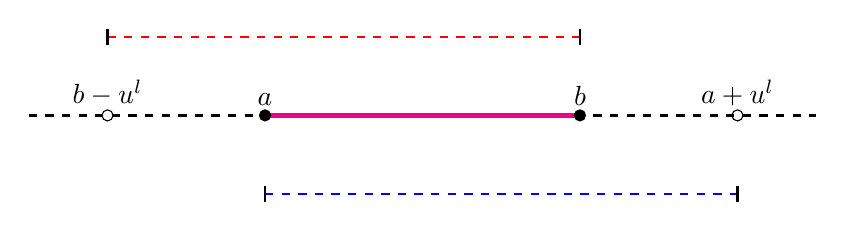
\begin{tikzpicture}
        \draw[dashed, blue, thick] (-2,0) -- (4,0);
        \draw[black, thick] (-2,-0.1) -- (-2,0.1);
        \draw[black, thick] (4,-0.1) -- (4,0.1);
        
        \draw[dashed, black, thick] (-5,1) -- (5,1);
        \draw[magenta, ultra thick] (-2,1) -- (2,1);
 
        
        \draw[dashed, red, thick] (-4,2) -- (2,2);
        
        \draw[black, thick] (-4,1.9) -- (-4,2.1);
        \draw[black, thick] (2,1.9) -- (2,2.1);
        
          
        \draw [black] (-4,1) circle (2pt) node[anchor=south] {$b-u^l$};

        \filldraw [black] (-2,1) circle (2pt) node[anchor=south] {$a$};

        \filldraw [black] (2,1) circle (2pt) node[anchor=south] {$b$};

        \draw [black] (4,1) circle (2pt) node[anchor=south] {$a+u^l$};
    \end{tikzpicture}
    \caption{Illustration of generalisation to arbitrary intervals $[a,b]$ for range proofs}
    \label{fig:interval}
\end{figure}


\subsection{Bulletproofs}
Bulletproof is a range proof, logarithmic in the size of the range. The proof relies on the inner product argument which allows a prove to convince a verifier that he knows the opening $\bm{s},\bm{q}\in\mathds{F}^n$ to a Pedersen vector commitment $P_v = \bm{g}^{\bm{s}}\bm{h}^{\bm{q}}$ such that the inner product of $\bm{s},\bm{q}$ is equal to a known value, $c$. This can be done with a proof of size $log\: n$, compare to the trivial solution of publishing $\bm{s},\bm{q}$ which is a proof of size $n$.

\subsubsection*{Notation and SetUp}
The description and construction of Bulletproofs uses some additional notation,  the notation used here is equivalent to the notation used in original Bulletproof paper, so for a detailed review of the notations please see this \cite{bulletProofs_theory} . 


% and will not be redefined instead the reader is encurraged to .  which will be presented here. First let lowercase bold font variables denote vectors, i.e $\mathbf{a}\in\mathds{F}^n$ is a vector with element $a_1,..,a_n \in \mathds{F}$, and uppercase bold font variables denote matrices, i.e $\mathbf{A}\in\mathds{F}^{n\times m}$ is a matrix and $a_{ij}$ the element of $\mathbf{A}$ at row $i$ and column $j$. Given this notation denote scalar multiplication with a vector as $\mathbf{b}=c\cdot \mathbf{a}\in\mathds{F}^n$, where $c\in\mathds{F}$ and  $b_i=c\cdot a_i, \: i\in\{1,...,n\}$. Denote the euclidean inner product of two vectors as $\langle \mathbf{a},\mathbf{b}\rangle$ and Hadamard product as $\mathbf{a}\circ \mathbf{b}$.

%Further consider vector polynomials $p(X)$ of degree $d$ on the form $p(X)=\sum_{i=0}^d \mathbf{p_i}\cdot X^i\in\mathds{F}^n[X]$, where the coefficients $\mathbf{p_i}\in\mathds{F}^n$. The inner product of two vector polynomials, $l(X),r(X)$ is defined as, 
%\begin{align*}
  %  \langle l(X),r(X)\rangle = \sum_{i=0}^d\sum_{j=0}^n \langle l_i,r_j\rangle \cdot X^{i+j}\in\mathds{F}[X].
%\end{align*}
%The following is equivalent: evaluating two polynomials at $x$ then taking the inner product versus taking the inner product polynomial at $x$.

%Let $\mathbf{a}||\mathbf{b}$ denote the concatenation of two vectors. Python notation will be used to denote sections of vectors such that $\mathbf{a}_{[:l]} = (a_1,...,a_l)$ and $\mathbf{a}_{[l:]} = (a_{l+1},...,a_n)$ for $l\in[1,n]$. 

%For $k\in\mathds{F}^*$ let $\mathbf{k}^n=(1,k,k^2,...,k^{n-1})$, i.e the vector containing the $n$ fist powers of $k$. 

%Let $\mathbf{g},\mathbf{h}\in\mathds{G}^n$ and remember that $\mathbf{a}\in\mathds{F}^n$ then define $C= \mathbf{g}^\mathbf{a} = \prod_{i=1}^ng_i^{a_i}\in\mathds{G}$, where $C$ can be interpreted as a commitment to the vector $\mathbf{a}$. In this section the two vectors $\mathbf{g},\mathbf{h}$ will be considered to be generators of the space $\mathds{G}^n$.


Remark that in this section $n$ will denotes the dimension of the room not the number of clients as earlier. Further remark that the dimension of the room is the length of the bit representation of the secret in the Pedersen vector commitment, potentially padded with zeros.

Both the construction of the inner product argument and the Bulletproof the parameters $g,h,\mathbf{g},\mathbf{h},u$ are assumed to be pre-shared and known by both verifier and prover. The assumptions about $g,h$ are before. Further the two vectors $\mathbf{g}, \mathbf{h} \in \mathds{G}^n$ are assumed to be independent generators of the space $\mathds{G}^n$. The variable $u\in\mathds{G}$ is such that there is no known discrete logarithm relation among $\mathbf{g},\mathbf{h}$. In order to ensure the fairness and correctness of the parameters $g,h,\mathbf{g},\mathbf{h},u$ they can be  assumed to be chosen by some trusted third party. Another possibility that drops the assumption of a trusted setup is to use the \textit{Nothing Up My Sleeve} (NUMS) strategy, \cite{ZKRP_Morais}.

\subsubsection*{Inner product argument}
\label{sec:inner_prod}
The Bulletproof construction is based on the inner product argument which will be closer presented in this section. The inner product argument is a argument of knowledge of $\textbf{s},\mathbf{q}$ in a  Pedersen vector commitment $P_v=\mathbf{g}^\mathbf{s}\mathbf{h}^\mathbf{q}$ satisfying a given inner product denoted $c$. 
%(To differ from the Pedersen vector commitment considered here and the Pedersen commitment in the range proofs the exponents in the commit are denoted $\mathbf{s},\mathbf{r}$ instead of $\sigma,R$, and the commitment by $P_v$) 
More formally the argument is a proof system of the statement,
\begin{align*}
    \{(\mathbf{g},\mathbf{h}\in\mathds{G}^n,\:P_v\in\mathds{G},\:c\in\mathds{F};\: \mathbf{s},\mathbf{q}\in\mathds{F}^n) : \: P_v=\mathbf{g}^\mathbf{s}\mathbf{h}^\mathbf{q}\wedge\: c =\langle\mathbf{s},\mathbf{q}\rangle\}
\end{align*}
Which can be shown to be equivalent to a proof of the statement,
\begin{align}
\label{eq:IPA}
    \{(\mathbf{g},\mathbf{h}\in\mathds{G}^n,\: u,P_v\in\mathds{G};\: \mathbf{s},\mathbf{q}\in\mathds{F}^n) : \: P_v=\mathbf{g}^\mathbf{s}\mathbf{h}^\mathbf{q}u^{\langle\mathbf{s},\mathbf{q}\rangle}\}.
\end{align}

A logarithmic sized proof of the above inner product statement is presented in Construction \ref{alg:inner_product}. The construction presented is modified compared to the one presented in \cite{bulletProofs_theory} to be non-interactive using the Fiat-Shamir heuristic.


\begin{algorithm}
\caption{\textbf{: Inner-product argument}}
\textbf{Goal:} Given a Pedersen vector  commitment $P_v=\bm{g}^{\bm{s}} \bm{h}^{\bm{q}}$ and a value $c$ prove that the two vectors $\bm{s},\bm{q}$ satisfies $\langle\bm{s},\bm{q}\rangle=c$.
\vspace{2pt}
\hline
\vspace{2pt}
\begin{itemize}
\item\text{\textbf{Prove} $(\mathbf{g},\mathbf{h},u,P_v,c,\mathbf{s},\mathbf{q})\xrightarrow[]{}\textit{proof}_{IP}$}\\
Let $y=\text{Hash}_{IP}(\mathbf{g},\mathbf{h},P_v,c) \in\mathds{F}^*$ and compute $P_v'= u^{y\cdot c}P$. Let $\mathbf{l},\mathbf{r}$ be two empty vectors. Run the recursive algorithm \textbf{GenerateProof}$(\mathbf{g},\mathbf{h},u^{x\cdot c},P_v,c,\mathbf{s},\mathbf{q},\mathbf{l},\mathbf{r})$ use the output $(g',h',u',P_v',s',q',\mathbf{l},\mathbf{r})$ to construct the inner product proof $\text{proof}_{IP} =(\mathbf{g},\mathbf{h},u',P_v,s',q',\mathbf{l},\mathbf{r} )$ and output $\textit{proof}_{IP}$. 
\item\text{\textbf{GenerateProof}$(\mathbf{g},\mathbf{h},u,P_v,\mathbf{s},\mathbf{q},\mathbf{l},\mathbf{r}) \xrightarrow[]{}  (g,h,u,P_v,s,q,\mathbf{l},\mathbf{r})$}
\begin{itemize}
    \item If the dimension of the vectors $\mathbf{g},\mathbf{h},\mathbf{s},\mathbf{q}$  drop the bold font and publish the proof $\textit{ proof}_{IP}=(g,h,P_v,u,s,q,\mathbf{l},\mathbf{r})$.
    \item  Otherwise:  Let $n'=n/2$ and define  $c_L=\langle \bm{s}_{[:,n']},\bm{q}_{[n',:]} \rangle$ and $c_R=\langle \mathbf{s}_{[n',:]},\mathbf{q}_{[:,n']} \rangle$. Then use these variables to calculate $L=\mathbf{g}_{[n':]}^{\mathbf{s}_{[:n']}} \mathbf{h}_{[:n']}^{\mathbf{q}_{[n':]}} u^{c_L}$ and $R=\mathbf{g}_{[:n']}^{\mathbf{s}_{[n':]}} \mathbf{h}_{[n':]}^{\mathbf{q}_{[:n']}} u^{c_R}$. Append  $L,R\in\mathds{G}$ to the vectors $\mathbf{l}$ resp $\mathbf{r}$. Now update $y=\text{Hash}_{BP}(L,R)$, and update $\mathbf{g}' = \mathbf{g}_{[:n']}^{y^{-1}}\mathbf{g}_{[n':]}^{y}$, $\mathbf{h}' = \mathbf{h}_{[:n']}^{y}\mathbf{h}_{[n':]}^{y^{-1}}$ and the commitment $P_v'=L^{y^2}PR^{y^{-2}}$. Finally update the vectors $\mathbf{s},\mathbf{q}$ to $\mathbf{s}' = \mathbf{s}_{[:n']}y+\mathbf{s}_{[n':]}y^{-1}$ and $\mathbf{q}' = \mathbf{q}_{[:n']}y^{-1}+\mathbf{q}_{[n':]}y$. Run the algorithm recursively, \textbf{GenerateProof}$(\mathbf{g}',\mathbf{h}',u,P_v',\mathbf{s}',\mathbf{q}',\mathbf{l},\mathbf{r})$ with the updated variables. Note that the vectors $\mathbf{g},\mathbf{h},\mathbf{s},\mathbf{q}$ now have the dimension $n'=n/2$, hence performing the recursion until one-dimensional vectors will require $log\:n$ iterations.
\end{itemize}
\item\text{\textbf{Verify} $(\textit{proof}_{IP} = (\mathbf{g},\mathbf{h},u,P_v,s,q,\mathbf{l},\mathbf{r}))\xrightarrow[]{}\{0,1\}$}\\
For $i\in\{0,log(n)\}$ put $n=n/2$ and $y=\text{Hash}(\bm{l}[i],\bm{r}[i])$, then update the vectors $\bm{g}$ and $\bm{h}$ as well as the  variable $P_v'$ according to, $\bm{g}'= \bm{g}_{[:,n]}^{y^{-1}} \bm{g}_{[n,:]}^{'y}$, $\bm{h}= \bm{h}_l{[:,n]}^{x}\bm{h}_{[n,:]}^{y^{-1}}$ and $ P_v' = L^{y^2}PR^{y^{-2}}  $. After iterating over all $i$ the dimension of the vectors $\bm{g},\bm{h}$ is one and we can drop the bold font. Compute  $c=\langle s, q\rangle$ and  accept if $P_v' =g^sh^ru^c$.
\end{itemize}
\label{alg:inner_product}
\end{algorithm}




%The setup phase of construction \ref{alg:inner_product} is intently left out since to avoid a trusted third party a \textit{Nothing up my sleeve} strategy will be used and is described separately in  section \ref{sec:NOMS}.
 
Remark that the inner product argument is sound but not zero-knowledge since information about two exponentials $\mathbf{s},\mathbf{q}$ is relieved.

\subsubsection*{Inner product rang proof}
Here the logarithmic sized range proof called \textit{Bulletproof}, based  on the inner product argument, is presented. This construction allows a prover, given a Pedersen commitment $C=g^x h^R$, of the secret $x$, to convince a verifier that the secret belongs to the interval $[0,2^n)$. By convincing the verifier that  $\bm{x}\in\{0,1\}^n$ is the binary representation of the secret $x$, or equivalently that $x= \langle \bm{x},\mathbf{2}^n\rangle $ and that the prover knows $\bm{x}$.
   % \item $\bm{\bar{x}}$ is the component-wise complement of $\bm{x}$. This is equivalent to show that $\bm{\bar{x}}$ satisfies the two conditions: $\bm{\bar{x}}\circ \bm{x}=\bm{0}^n$ and $\bm{\bar{x}} = \bm{x} -\bm{1}^n \: \text{mod }2$.
%\end{itemize}
This can be shown to be done by proving the following statement;
\begin{align}
    \big\langle \bm{x} -z\cdot \bm{1}^n, \bm{y}^n\circ (\bm{\bar{x}} + z \cdot\bm{1}^n) + z^2\cdot\bm{2}^n \big\rangle = z^2\cdot x+ \delta(y,z),
    \label{eq:range_non_zero}
\end{align}
where $\bar{\bm{x}}$ is the component-wise complement of $\bm{x}$ and $\delta(y,z) = (z-z^2)\cdot\langle\bm{1}^n,\bm{y}^n\rangle-z^3\langle \bm{1}^n,\bm{2}^n\rangle\in\mathds{F}$.
The values $z$ and $y$ are either chosen at random from the set $\mathds{F}$ by the verifier in an interactive construction or are the output of a hash function in a non-interactive construction. Here a non-interactive construction will be considered. 

Directly using  a inner product argument presented in Construction \ref{alg:inner_product} to prove the statement  in equation \eqref{eq:range_non_zero} would leak information about $x$, since information about the two vectors $\bm{x},\bm{\bar{x}}$ is revealed, i.e the binary representation of $x$. Hence two new vectors $\bm{s}_1,\bm{s}_2$ are introduced and will serve as blinding vectors and help construct a zero-knowledge range proof even if the inner product argument is not a zero knowledge construction. Given this idea, the inner product in \eqref{eq:range_non_zero} is tweaked to include the two blinding vectors and the new statement is to prove the inner product of is,
\begin{align*}
     t(X) &= \langle  l(X),r(X)\rangle = t_0 + t_1\cdot X + t_2\cdot X^2\\
    l(X) &= \bm{x} -z\cdot \bm{1}^n +\bm{s}_1\cdot X\\
    r(X) &= \bm{y}^n\circ (\bm{\bar{x}} + z \cdot\bm{1}^n + \bm{s}_2\cdot X)+ z^2\cdot\bm{2}^n,\\
\end{align*}
Note that $t_0 = z^2 \cdot x + \delta(y,z)$ which is equal to the right hand side of equation \eqref{eq:range_non_zero}. Further it holds that $t_1 = \langle \bm{x}-z\cdot \bm{1}^n , \bm{y}^n\circ \bm{s_R}\rangle + \langle\bm{s_L},\bm{y}^n\circ (\bm{a_R}+z\cdot\bm{1}^n) + z\cdot \bm{2}^n\rangle$ and $t_2 =\langle \bm{s_L}, \bm{y}^n \circ \bm{s_R}\rangle $. Given these vectors and innner product Construction \ref{alg:bullet} gives a non interactive zero knowledge range proof that the secret $x$ belongs to the interval $[0,2^n]$.

\begin{algorithm}[]
\caption{\textbf{: Bulletproof}}
\textbf{Goal:}  Given a Pedersen commitment $C=g^x h^R$ and a number $n$, prove that the secret $x$ in the commitment belongs to the range  $[0,2^n)$ without revealing anything else about $x$.
\vspace{2pt}
\hline
\vspace{2pt}
\begin{itemize}
\item\text{\textbf{Prove} $(g,h,\mathbf{g},\mathbf{h},P,n,x,R,u)\xrightarrow[]{}\textit{ proof}_{RP}$}\\
Let $\bm{x}$ denote the binary representation of the secret $x$ in the commitment $P$ and $\bar{\bm{x}}$ the component-wise complement such  that $\bm{x}\circ \bar{\bm{x}} = 0$. Construct the commitment $A= h^{\alpha} \bm{g}^{ \bm{x} } \bm{h}^{ \bar{\bm{x}} }$, where $\alpha \in_R \mathds{F}$. Then chose the two blinding vectors $\bm{s_R},\bm{s_L}\in_R\mathds{F}^n$ and the value $\rho\in_R\mathds{F}$ and compute the commitment $S=h^{\rho} \bm{g}^{\bm{s_L}} \bm{h}^{\bm{s_R}}$. Let $y=\text{Hash}(A,S)$, $z=\text{Hash}(A,S,y)$ and $\tau_1,\tau_2\in_R\mathds{F}$. Now the it is possible to construct $t_1,t_2$ defined above. Given this let $T_1=g^{t_1}h^{\tau_1}$ and $T_2=g^{t_2}h^{\tau_2}$, next let $X=\text{Hash}(T_1,T_2)$. Now construct the two vectors for the inner product argument: $\bm{l} = \bm{x}-z\cdot \bm{1}^n-\bm{s_L}\cdot X$, $\bm{r}= \bm{y}^n\circ(\bar{\bm{x}}+ z\cdot \bm{1}^n+\bm{s_R}\cdot X ) + z^2\ X $ and calculate the inner product $\hat{t} = \langle \bm{l},\bm{r}\rangle$. Finally compute $\tau_X = \tau_2 x^2 + \tau_1 X + z^2 R$ and $\mu = \alpha+ R\:X$.  Now use the inner product argument to prove that $\hat{t}$ is indeed the inner product of the two vectors $\mathbf{l},\mathbf{r}$ using the commitment $P_v = \bm{g}^{\bm{l}}\bm{h}^{\bm{r}}$, run the algorithm  \textbf{Prove}  defined Construction \ref{alg:inner_product} with the input $(\bm{g},\bm{h},u,P_v,\hat{t},\bm{l},\bm{r})$ to construct such a proof denoted  \textit{proof$_{IP}$}. Combine and publish  the proof: $\textit{proof}_{RP} = (\tau_X, \mu , \hat{t}, P, A, S, T_1, T_2 , P_v ,\textit{proof}_{IP}) $.

\item\text{\textbf{Verify} $(g,h,C,\textit{proof}_{RP})\xrightarrow[]{}\{0,1\}$}\\
Compute the three hash functions $y= \text{Hash}(A,S)$, $z= \text{Hash}(A,S,y)$ and $X= \text{Hash}(T_1,T_2)$. Then given  $y,z,X$ compute $h_i' = h_i ^{y^{-i+1}}$ for all $i\in\{1,...,n\}$, $P_l = P\cdot h\mu$ and $P_r = A\cdot S ^x \bm{g}^ {-z}\bm{h'}^{z\bm{y}^n+z^2\cdot \bm{2}^n}$. Then check if the following equalities hold: $P_l\overset{?}{=} P_r \wedge g^{\hat{t}}h^{\tau_X} \overset{?}{=}  P ^{z^2}\:g^{\delta(y,z)}\:T_1^x\:T_2^{x^2}$ and if the output of \textbf{Verify} in Construction \ref{alg:inner_product} on the input $(\text{proof}_{IP})$ is $1$. If all three criterion is fulfilled then the secret  $x$ in the commitment $P$ is in the range $[0,2^n]$.
\end{itemize}
\label{alg:bullet}
\end{algorithm}

%Bulletproofs can be modified to prove that a secret belongs to an arbitrary range, $[a,b]$, with a similar approach as presented for the signature based range proofs and illustrated in Figure \ref{fig:interval}. Remember that the range cannot be completely arbitrary it must hold that $a>0$ and $b>a$. A Bulletproof where one prover wishes to verify the range of several commitments can be optimised such that the  proof size does not growing multiplicatively in the number of commits but instead grows additive. More precisely lets a assume a prover wants to prove the range of $k$ commits a naive implementation would lead to a proof size of $k\cdot log_2 n $, but an optimised implementation reduces this to $log_2 n + 2 log_2 k$.  Hence for the case of arbitrary intervals  proof size is increased with the additive term $2log_2 2 = 2$. 


%Optimise when one proving much!
%Vad för hash function? 
%Se igenom notation både generell  o bullet

